\documentclass{report}
\usepackage[a4paper,total={7in,10in}]{geometry}

\usepackage{amsmath}
\usepackage{amssymb}
\usepackage{enumitem}
\usepackage{tikz, pgfplots}
\usepackage{multicol}
\usepackage{setspace}
\usepackage{graphicx}
\usetikzlibrary{arrows}

\setcounter{chapter}{10}
\setcounter{section}{2}

\newcommand{\sol}{\vspace{1em}\\\textbf{Sol.}}
\newcommand{\proof}{\vspace{1em}\\\textbf{Proof.}}
\newcommand{\eos}{ \qquad \square}

\begin{document}
\section*{Exercise 5c}

\onehalfspacing
\begin{enumerate}[leftmargin=*]
    \item Find the standard form of the equation of the ellipse that satisfies the given
          conditions:
          \begin{enumerate}
              \item Passes through point $P(-2\sqrt{2}, 0)$, $Q(0, \sqrt{5})$; \sol{}

                    Point $P$ is on the $x$-axis, while point $Q$ is on the $y$-axis.

                    $|OP| = 2\sqrt{2}$, $|OQ| = \sqrt{5}$,

                    $\because$ $|OP| > |OQ|$,

                    $\therefore$ The major axis is along the $x$-axis.

                    $\therefore$ The equation of the ellipse is of the form
                    \begin{align*}
                        \frac{x^2}{a^2} + \frac{y^2}{b^2} = 1
                    \end{align*}

                    Substituting the coordinates of $P$ and $Q$ into the equation, we get
                    \begin{align*}
                        \frac{(-2\sqrt{2})^2}{a^2} + \frac{0^2}{b^2} & = 1 \\
                        \frac{0^2}{a^2} + \frac{(\sqrt{5})^2}{b^2}   & = 1
                    \end{align*}
                    Simplifying, we get
                    \begin{align*}
                        \frac{8}{a^2} & = 1 \\
                        \frac{5}{b^2} & = 1
                    \end{align*}
                    Solving for $a$ and $b$, we get
                    \begin{align*}
                        a^2 & = 8 \\
                        b^2 & = 5
                    \end{align*}
                    $\therefore$ The standard form of the equation of the ellipse is
                    \begin{align*}
                        \frac{x^2}{8} + \frac{y^2}{5} = 1 \eos
                    \end{align*}
                    \vspace{1em}
                    \begin{center}
                        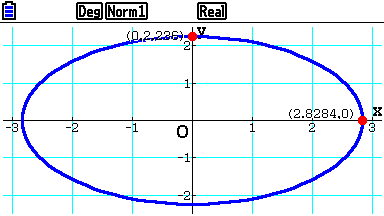
\includegraphics[scale=0.7]{./assets/ex5c1a.png}
                    \end{center}

                    \newpage
              \item Coordinates of its foci are $(-2\sqrt{3}, 0)$ and $(2\sqrt{3}, 0)$, and it
                    passes through the point $P(\sqrt{5}, -\sqrt{6})$;

                    The foci are on the $x$-axis, therefore let the equation of the ellipse be of
                    the form
                    \begin{align*}
                        \frac{x^2}{a^2} + \frac{y^2}{b^2} = 1
                    \end{align*}
                    From the coordinates of the foci, we have
                    $ae = 2\sqrt{3}$, $a^2e^2 = 12$,
                    \begin{align*}
                        \therefore\ b^2 & = a^2 - a^2e^2          \\
                                        & = a^2 - 12\ \cdots\ (1)
                    \end{align*}
                    Substituting the coordinates of $P$ into the equation $\dfrac{x^2}{a^2} + \dfrac{y^2}{b^2} = 1$, we get
                    \begin{align*}
                        \frac{(\sqrt{5})^2}{a^2} + \frac{(-\sqrt{6})^2}{b^2} & = 1 \\
                        \frac{5}{a^2} + \frac{6}{b^2}                        & = 1
                    \end{align*}
                    Substituting $(1)$ into the equation, we get
                    \begin{align*}
                        \frac{5}{a^2} + \frac{6}{a^2 - 12} & = 1                                           \\
                        5(a^2 - 12) + 6a^2                 & = a^2(a^2 - 12)                               \\
                        5a^2 - 60 + 6a^2                   & = a^4 - 12a^2                                 \\
                        a^4 - 23a^2 + 60                   & = 0                                           \\
                        (a^2 - 20)(a^2 - 3)                & = 0                                           \\
                        a^2 = 20\                          & \text{or}\ a^2 = 3\ (\text{rejected, } b > 0)
                    \end{align*}
                    When $a^2 = 20$, $b^2 = 20 - 12 = 8$.
                    $\therefore$ The standard form of the equation of the ellipse is
                    \begin{align*}
                        \frac{x^2}{20} + \frac{y^2}{8} = 1 \eos
                    \end{align*}
                    \vspace{1em}
                    \begin{center}
                        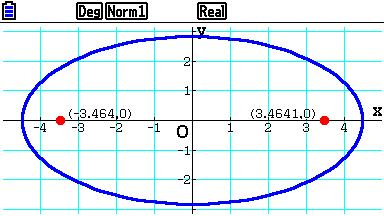
\includegraphics[scale=0.7]{./assets/ex5c1b.png}
                    \end{center}

                    \newpage
              \item Equations of its directrices are $y \pm \dfrac{25}{3} = 0$, and it passes
                    through the point $(4, 0)$; \sol{}

                    The directrices are perpendicular to the $y$-axis, therefore let the equation
                    of the ellipse be of the form
                    \begin{align*}
                        \frac{x^2}{b^2} + \frac{y^2}{a^2} = 1
                    \end{align*}
                    From the equation of the directrices, we have
                    $\dfrac{a}{e} = \dfrac{25}{3}$, $\dfrac{a^2}{e^2} = \dfrac{625}{9}$, $e^2 = \dfrac{9}{625}a^2$,
                    \begin{align*}
                        \therefore\ b^2 & = a^2 - a^2e^2                        \\
                                        & = a^2 - \frac{9}{625}a^4\ \cdots\ (1)
                    \end{align*}
                    Substituting the point $(4, 0)$ into the equation $\dfrac{x^2}{b^2} + \dfrac{y^2}{a^2} = 1$, we get
                    \begin{align*}
                        \frac{(4)^2}{b^2} + \frac{0^2}{a^2} & = 1 \\
                        \frac{16}{b^2}                      & = 1
                    \end{align*}
                    Substituting $(1)$ into the equation, we get
                    \begin{align*}
                        \frac{16}{a^2 - \dfrac{9}{625}a^4} & = 1                            \\
                        16                                 & = a^2 - \frac{9}{625}a^4       \\
                        9a^4 - 625a^2 + 10000              & = 0                            \\
                        (9a^2 - 400)(a^2 - 25)             & = 0                            \\
                        a^2 = 25\                          & \text{or}\ a^2 = \frac{400}{9}
                    \end{align*}
                    When $a^2 = 25$, $b^2 = 25 - \dfrac{9}{625}(25)^2 = 25 - 9 = 16$.

                    When $a^2 = \dfrac{400}{9}$, $b^2 = \dfrac{400}{9} -
                        \dfrac{9}{625}\left(\dfrac{400}{9}\right)^2 = 16$.

                    $\therefore$ The standard form of the equations of the ellipse is
                    \begin{align*}
                        \frac{x^2}{16} + \frac{y^2}{25} = 1\qquad \text{ or } \qquad \frac{x^2}{16} + \frac{9y^2}{400} = 1 \eos
                    \end{align*}

                    \newpage
              \item Its eccentricity is $\dfrac{4}{5}$ while the distance between its two foci is
                    8. \sol{}

                    Let the equation of the ellipse be of the forms
                    \begin{align*}
                        \frac{x^2}{a^2} + \frac{y^2}{b^2} = 1\qquad \text{ or } \qquad \frac{x^2}{b^2} + \frac{y^2}{a^2} = 1
                    \end{align*}
                    From the given information, we have
                    \begin{align*}
                        \sqrt{(2ae)^2 - 0^2}             & = 8                         \\
                        2ae                              & = 8                         \\
                        ae                               & = 4\ \cdots\ (1)            \\
                        e = \dfrac{1}{a}\sqrt{a^2 - b^2} & = \dfrac{4}{5}\ \cdots\ (2)
                    \end{align*}
                    Substituting $(2)$ into $(1)$, we get
                    \begin{align*}
                        \frac{4}{5}a & = 4 \\
                        a            & = 5
                    \end{align*}
                    Substituting $a = 10$ into $(2)$, we get
                    \begin{align*}
                        \dfrac{1}{5}\sqrt{5^2 - b^2} & = \dfrac{4}{5} \\
                        \sqrt{25 - b^2}              & = 4            \\
                        25 - b^2                     & = 16           \\
                        b^2                          & = 9            \\
                        b                            & = 3\ (b > 0)
                    \end{align*}
                    $\therefore$ The standard form of the equation of the ellipse is
                    \begin{align*}
                        \frac{x^2}{25} + \frac{y^2}{9} = 1\qquad \text{ or } \qquad \frac{x^2}{9} + \frac{y^2}{25} = 1 \eos
                    \end{align*}
                    \vspace{1em}
                    \begin{center}
                        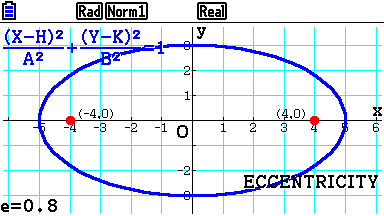
\includegraphics[scale=0.5]{./assets/ex5c1d1.png}
                        \hspace{1em}
                        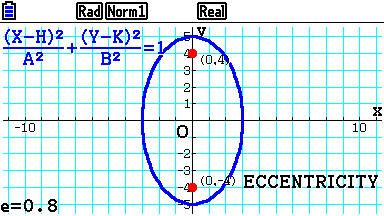
\includegraphics[scale=0.5]{./assets/ex5c1d2.png}
                    \end{center}
          \end{enumerate}

          \newpage
    \item The two vertices of one of the sides of the triangle $\triangle ABC$ is $B(0,
              6)$ and $C(0, -6)$, while the product of the slopes of the other two sides is
          $-\dfrac{4}{9}$, find the equation of the locus of the point $A$. \sol{}

          Let point $A$ be $(x, y)$.
          \begin{align*}
              \text{Slope of } AB & = \frac{y - 6}{x - 0} = \frac{y - 6}{x} \\
              \text{Slope of } AC & = \frac{y + 6}{x - 0} = \frac{y + 6}{x}
          \end{align*}
          The product of the slopes of $AB$ and $AC$ is
          \begin{align*}
              \frac{y - 6}{x} \cdot \frac{y + 6}{x} & = -\frac{4}{9} \\
              \frac{y^2 - 36}{x^2}                  & = -\frac{4}{9} \\
              9y^2 - 324                            & = -4x^2        \\
              9y^2 + 4x^2                           & = 324          \\
              \dfrac{x^2}{81} + \dfrac{y^2}{36}     & = 1 \eos
          \end{align*}

    \item The ratio between point $M$ and the two foci of the ellipse $\dfrac{x^2}{13^2}
              + \dfrac{y^2}{12^2} = 1$ is $\dfrac{2}{3}$, find the equation of the locus of
          point $M$. Hence, sketch the graph. \sol{}

          The eccentricity of the ellipse is
          \begin{align*}
              e & = \dfrac{1}{13}\sqrt{13^2 - 12^2} = \dfrac{5}{13}
          \end{align*}
          $\therefore$ The foci of the ellipse are at $(\pm 5, 0)$.

          Let point $M$ be $(x, y)$.
          \begin{align*}
              \sqrt{(x - 5)^2 + y^2}   & = \dfrac{2}{3}\sqrt{(x + 5)^2 + y^2} \\
              (x - 5)^2 + y^2          & = \dfrac{4}{9}[(x + 5)^2 + y^2]      \\
              9(x - 5)^2 + 9y^2        & = 4(x+5)^2 + 4y^2                    \\
              9x^2 - 90x + 225 + 9y^2  & = 4x^2 + 40x + 100 + 4y^2            \\
              5x^2 - 130x + 125 + 5y^2 & = 0                                  \\
              x^2 + y^2 - 26x + 25     & = 0 \eos
          \end{align*}
          \vspace{1em}
          \begin{center}
              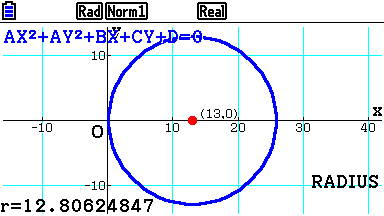
\includegraphics[scale=0.5]{./assets/ex5c3.png}
          \end{center}

          \newpage
    \item Find the distance between a point $M\left(\dfrac{12}{5}, 4\right)$ on the
          ellipse $\dfrac{x^2}{16} + \dfrac{y^2}{25} = 1$ and the foci of the ellipse.
          \sol{}

          The eccentricity of the ellipse is $e = \dfrac{1}{5}\sqrt{25 - 16} =
              \dfrac{3}{5}$.

          Hence, the foci $F$ and $F'$ of the ellipse are at $(0, 3)$ and $(0, -3)$
          respectively.
          \begin{align*}
              |MF|  & = \sqrt{\left(\frac{12}{5} - 0\right)^2 + (4 - 3)^2} = \sqrt{\frac{144}{25} + 1} = \frac{13}{5} \eos     \\
              \\
              |MF'| & = \sqrt{\left(\frac{12}{5} - 0\right)^2 + (4 - (-3))^2} = \sqrt{\frac{144}{25} + 49} = \frac{37}{5} \eos
          \end{align*}

    \item Lazy to do this one. =)
    \item Find the equation of the ellipse of which the length of its minor axis is 8 and
          its foci are $(1, 5)$ and $(4, 5)$. \sol{}

          The center of the ellipse is at $\left(\dfrac{4 + 1}{2}, 5\right) =
              \left(\dfrac{5}{2}, 5\right)$.

          Translate the coordinates system so that the center of the ellipse is at the
          origin, we obtain a new set of coordinates $(x', y')$ such that
          \begin{align*}
              x' & = x - \frac{5}{2}\qquad y' = y - 5
          \end{align*}
          Since the foci are on the $x$-axis, the equation of the ellipse is of the form $\dfrac{x'^2}{a^2} + \dfrac{y'^2}{b^2} = 1$

          The coordinates of the loci in the new coordinates system are
          $\left(-\dfrac{3}{2}, 0\right)$ and $\left(\dfrac{3}{2}, 0\right)$.
          \begin{align*}
              ae = \frac{3}{2}  & \implies e = \frac{3}{2a}      \\
              e                 & = \dfrac{1}{a}\sqrt{a^2 - 16}  \\
              \dfrac{3}{2a}     & = \dfrac{1}{a}\sqrt{a^2 - 16}  \\
              2a\sqrt{a^2 - 16} & = 3a                           \\
              4a^2(a^2 - 16)    & = 9a^2                         \\
              4a^4 - 64a^2      & = 9a^2                         \\
              a^2(4a^2 - 73)    & = 0                            \\
              a^2 = 0           & \text{ or } a^2 = \frac{73}{4} \\
              a                 & = \sqrt{\frac{73}{4}}\ (a > 0)
          \end{align*}
          $\therefore$ The standard form of the equation of the ellipse is $\dfrac{4x'^2}{73} + \dfrac{y'^2}{16} = 1$.

          Substituting $x' = x - \dfrac{5}{2}$ and $y' = y - 5$ into the equation, we get
          \begin{align*}
              \frac{4(x - \dfrac{5}{2})^2}{73} + \frac{(y - 5)^2}{16} & = 1 \eos
          \end{align*}

    \item Find the equation of the ellipse of which the length of its minor axis is
          $2\sqrt{2}$ and the two ends of its major axis are at $(-2, 2)$ and $(8, 2)$.
          \sol{}

          The center of the ellipse is at $\left(\dfrac{-2 + 8}{2}, 2\right) = (3, 2)$.

          Translate the coordinates system so that the center of the ellipse is at the
          origin, we obtain a new set of coordinates $(x', y')$ such that
          \begin{align*}
              x' & = x - 3\qquad y' = y - 2
          \end{align*}

          Since the major axis is along the $x$-axis, the equation of the ellipse is of
          the form $\dfrac{x'^2}{a^2} + \dfrac{y'^2}{b^2} = 1$

          The length of the major axis is $8 - (-2) = 10$, therefore $2a = 10$, $a = 5$.

          The length of the minor axis is $2\sqrt{2}$, therefore $2b = 2\sqrt{2}$, $b =
              \sqrt{2}$.

          $\therefore$ The standard form of the equation of the ellipse is $\dfrac{x'^2}{25} + \dfrac{y'^2}{2} = 1$.

          Substituting $x' = x - 3$ and $y' = y - 2$ into the equation, we get
          \begin{align*}
              \frac{(x - 3)^2}{25} + \frac{(y - 2)^2}{2} & = 1 \eos
          \end{align*}

    \item The orbit of the earth is an ellipse with half major axis of length $a = 1.50
              \times 10^8$ km, eccentricity $e = 0.0192$, and the sun at one of its foci.
          Find the maximum and the minimum distance of the earth from the sun. \sol{}
          \begin{align*}
              ae & = 1.50 \times 10^8 \times 0.0192 = 2.88 \times 10^6 \text{ km}
          \end{align*}
          The maximum distance of the earth from the sun is $a + ae = 1.50 \times 10^8 + 2.88
              \times 10^6 = 1.5288 \times 10^8$ km.

          The minimum distance of the earth from the sun is $a - ae = 1.50 \times 10^8 -
              2.88 \times 10^6 = 1.4712 \times 10^8$ km. $\eos$

    \item Find the eccentricity of the following ellipses:
          \begin{enumerate}
              \item The view angle from the focus to the two ends of the minor axis is $60^\circ$.
                    \sol{}

                    The angle between the major axis and the line joining the foci is $30^\circ$.
                    \begin{align*}
                        \dfrac{b}{ae} & = \tan 30^\circ = \dfrac{1}{\sqrt{3}} \\
                        b             & = \dfrac{ae}{\sqrt{3}}                \\
                        a^2e^2        & = 3b^2                                \\
                        a^2e^2        & = 3[a^2(1 - e^2)]                     \\
                                      & = 3a^2 - 3a^2e^2                      \\
                        e^2           & = 3 - 3e^2                            \\
                        4e^2          & = 3                                   \\
                        e^2           & = \dfrac{3}{4}                        \\
                        e             & = \dfrac{\sqrt{3}}{2}\ (e > 0) \eos
                    \end{align*}

              \item The viewing angle from one end of the minor axis to the foci is straight angle.
                    \sol{}

                    Let the coordinates of the foci be $(\pm ae, 0)$, and the coordinates of one of
                    the ends of the minor axis be $(0, b)$.

                    The slope of the lines joining the foci and the end of the minor axis is
                    $\dfrac{b}{ae}$ and $\dfrac{-b}{ae}$.

                    Since the two lines are perpendicular, we have
                    \begin{align*}
                        \dfrac{b}{ae} \cdot \dfrac{-b}{ae} & = -1                                \\
                        \dfrac{-b^2}{a^2e^2}               & = -1                                \\
                        -b^2                               & = -a^2e^2                           \\
                        a^2 - a^2e^2                       & = a^2e^2                            \\
                        2e^2                               & = 1                                 \\
                        e^2                                & = \dfrac{1}{2}                      \\
                        e                                  & = \dfrac{\sqrt{2}}{2}\ (e > 0) \eos
                    \end{align*}
          \end{enumerate}

    \item Calculate the side length of the inscribed square in the ellipse
          $\dfrac{x^2}{a^2} + \dfrac{y^2}{b^2} = 1$. \sol{}

          Let one of the vertices of the square that is in the first quadrant be $(m,
              m)$.

          Substituting the coordinates of the vertex into the equation of the ellipse, we
          get
          \begin{align*}
              \frac{m^2}{a^2} + \frac{m^2}{b^2}             & = 1                           \\
              m^2\left(\frac{1}{a^2} + \frac{1}{b^2}\right) & = 1                           \\
              m^2                                           & = \frac{a^2b^2}{a^2 + b^2}    \\
              m                                             & = \frac{ab}{\sqrt{a^2 + b^2}}
          \end{align*}
          Hence, the side length of the inscribed square is $\dfrac{2ab}{\sqrt{a^2 + b^2}} = \dfrac{2ab}{a^2 + b^2}\sqrt{a^2 + b^2}$. $\eos$

    \item Prove that the points of intersection of the two ellipses $b^2x^2 + a^2y^2 -
              a^2b^2 = 0$ and $a^2x^2 + b^2y^2 - a^2b^2 = 0$ ($a > b > 0$) are on the
          circumference of a circle with the center at the origin. Hence, find the
          equation of the circle. \proof{}

          Adding the two equations, we get
          \begin{align*}
              b^2x^2 + a^2y^2 - a^2b^2 + a^2x^2 + b^2y^2 - a^2b^2 = 0 \\
              (a^2 + b^2)x^2 + (a^2 + b^2)y^2 - 2a^2b^2 = 0           \\
              x^2 + y^2 & = \frac{2a^2b^2}{a^2 + b^2} \eos
          \end{align*}

\end{enumerate}
\end{document}